%Preamble
\documentclass[12pt,a4paper]{article}        %Define text type and basic formatting
%\usepackage[document]{ragged2e}   %Text alignment https://www.overleaf.com/learn/latex/Text_alignment

\usepackage[utf8]{inputenc}     %Usage of UTF-8 for umlauts
\usepackage[ngerman]{babel}     %Paper language;
\pagenumbering{arabic}  % "Normal" page numbering
%Set line spacing to 1.5
% \usepackage{setspace}
% \onehalfspacing

%Citation and reference
\usepackage[backend=biber,
  style=authoryear,
  citestyle=authoryear-comp,
  hyperref=true,
  giveninits,    %Shorten first names to initial
  uniquename=init,    %prevent name disambiguation
  sorting=nyt,  % sort by name, year, title
  natbib,  %enable citep/citet(parentheses only around year)
  maxbibnames=99,  %show all names in bibliography (no influence on in-text citation)
  minbibnames=1  %show at least one name before et al
]{biblatex}   %REFERENCES https://www.overleaf.com/learn/latex/Bibliography_management_in_LaTeX
\addbibresource{references.bib}     %Lib file
\usepackage[nottoc,numbib]{tocbibind}   %add bibliography to toc

%page citation in text with colon: https://tex.stackexchange.com/questions/433122/changing-comma-in-textcite-to-colon
%\DeclareFieldFormat{postnote}{#1}
%\DeclareFieldFormat{multipostnote}{#1}
%\renewcommand\postnotedelim{\addcolon\addspace}
\renewcommand\nameyeardelim{\addcomma\space} %comma between author and year
%u.a. as et al.
\DefineBibliographyStrings{german}{%
  andothers = {et al.},
}
%Replace and/und with &
\renewcommand*{\finalnamedelim}{%
  \ifnumgreater{\value{liststop}}{2}{\finalandcomma}{}%
\addspace\&\space}%

%images
\usepackage{graphicx}       %Required for adding images
\graphicspath{{images/}}    %image path
\usepackage{wallpaper}  %Page background img

\usepackage{parskip}        %Prevent indention of paragraphs
\usepackage{mathtools}    %required for math formulas
\usepackage{amssymb}    %mathematical symbols
\usepackage{listings}   %For code listings

%Use markdown in LaTex https://de.overleaf.com/learn/latex/Articles/How_to_write_in_Markdown_on_Overleaf
\usepackage[footnotes,definitionLists,hashEnumerators,smartEllipses,hybrid]{markdown}

\usepackage{titlesec}   %Style titles
\usepackage{fancyhdr}   %Header/footer
%\usepackage[bottom]{footmisc}   %Foot notes, at end of page

%Links
\usepackage[colorlinks,
  pdfpagelabels,
  pdfstartview = FitH,
  bookmarksopen = true,
  bookmarksnumbered = true,
  linkcolor = black,
  plainpages = false,
  hypertexnames = false,
  citecolor = black,
urlcolor = black]{hyperref}   %Hyperref pkg -> clickable links and TOC
\usepackage{csquotes}   % Autostyle quotes language-specific

%Font settings
\renewcommand{\familydefault}{\sfdefault}       %Text sans-serif
\renewcommand{\headrulewidth}{0pt}
\pagestyle{fancy}

%Footer
\fancyhf{}      %Clear all header/footer stylings
% \lfoot{\thedate\hspace{1pt}}
% \cfoot{Proposal Bachelorarbeit\\«Video- und bildbasierte Desinformation auf Social-Media-Plattformen in der Schweiz» (Arbeitstitel)} % Footnote
\rfoot{\thepage\hspace{1pt}}        %Add page number

%Title page settings
\usepackage{pdfpages}
\usepackage{titling}    %Title page styling
\title{«Analyse (audio-) visueller Desinformation auf Social-Media-Plattformen in der Schweiz» (Arbeitstitel)}        %Document Title
\author{Yannick Spriessler}     %Author of paper
\date{\today}     %Date of paper; ALTERNATIVE: \today

% Separate bibliography for images
% \defbibheading{imagecredits}{\section*{Bildverweis}}
% \addbibresource{img-references.bib}

%___________________________________________________________________________________________
%TITLE PAGE
\begin{document}
\begin{titlingpage} %Start titling page
  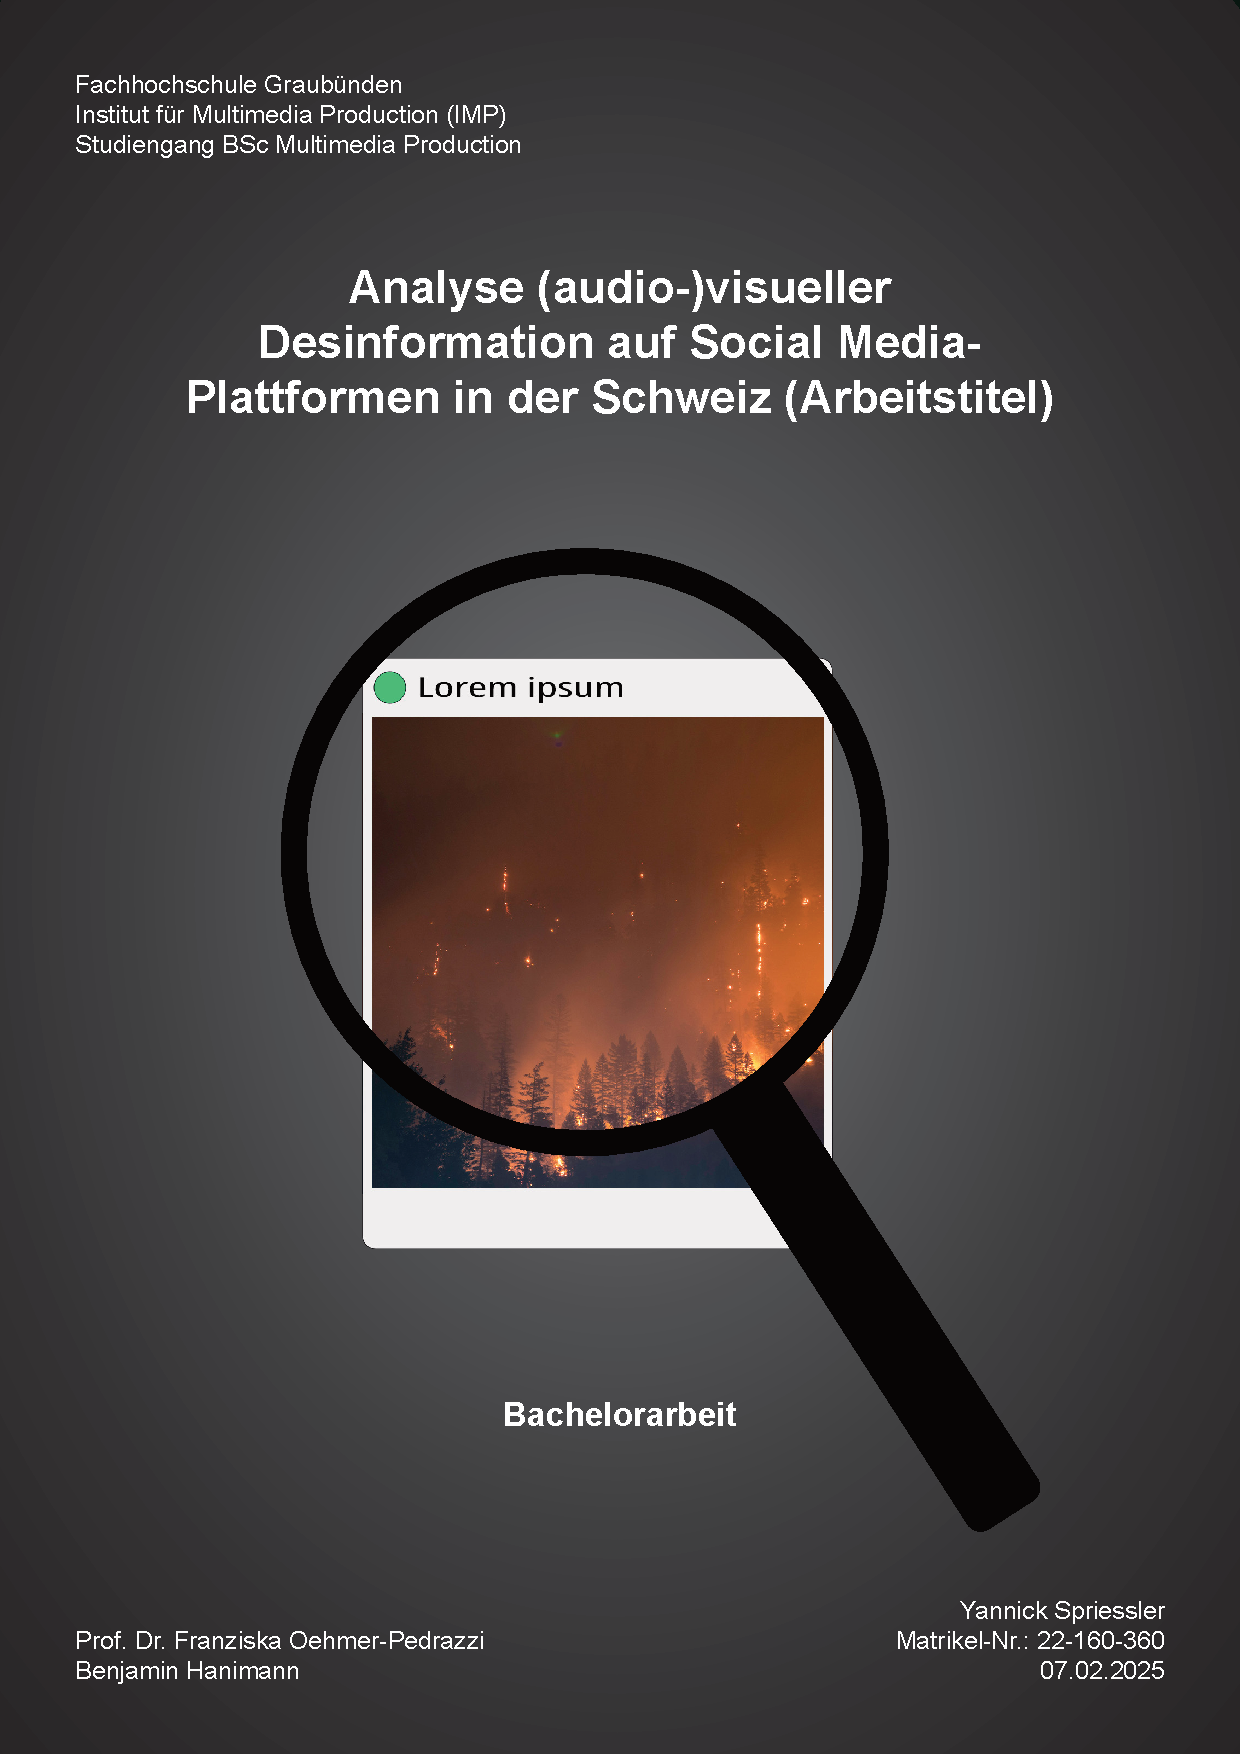
\includepdf{Titelblatt_Thesis}
  \nocite{howard_trees_2017}  %Citation for title page, only in image bibliography
\end{titlingpage}
\pagebreak      %Insert page break
%-----------------------------------------------
%TOC
\thispagestyle{empty}
\setcounter{page}{0}    %Set page no.
\tableofcontents        %Content index
\pagebreak
%-----------------------------------------------
%DOC
\renewcommand{\abstractname}{Abstract}
\begin{abstract}
  \setlength{\parindent}{0pt}  
    asdfghjk \\
\end{abstract}

\textbf{Keywords:} \textit{Desinformation, Social Media, audiovisuelle Inhaltsanalyse}


\textbf{Zitiervorschlag:}
\linebreak
%\frontmatter   %If foreword
\pagebreak

%\mainmatter    %Main part if foreword used
\section{Einleitung}
Spätestens seit den US-Wahlen 2016 hat der Begriff «Fake News» stark an Bedeutung gewonnen. Zwar handelt es sich dabei nicht um eine Neuerscheinung und falsche Informationen wurden lange vor der Entwicklung des Internets verbreitet \parencites[214]{allcott_social_2017}[247]{hohlfeld_schlechte_2020}[1]{khan_fake_2021}, dennoch ist das Problem unter anderem durch die Verbreitung über das Internet weiter stark angewachsen \parencites[214–215]{allcott_social_2017}[1]{khan_fake_2021}[1]{lazer_science_2018}[4]{ceron_fake_2021}. \\
Aufgrund der sozialen Medien und der Möglichkeit, innerhalb kürzester Zeit Videos und Bilder zu produzieren, können heute sehr schnell audiovisuelle Falschinformationen verbreitet werden. Diese stellen nicht nur ein Problem für die individuellen EmpfängerInnen dar, sondern gefährden dabei auch politische und gesellschaftliche Prozesse.

Die Bachelorarbeit befasst sich damit, welche inhaltlichen und gestalterischen Merkmale audiovisuelle und bildbasierte Desinformation auf Social-Media-Plattformen in der Schweiz aufweist. \\
Ziel der Arbeit ist es zum einen herauszufinden, ob es mögliche Muster und
Strategien hinter der Produktion der Inhalte gibt. Zum anderen soll auch ein
allgemeines Verständnis über die entsprechenden Inhalte gewonnen werden. \\
Die Erkenntnisse der Bachelorarbeit werden anschliessend verwendet, um darauf basierend eine interaktive Aufklärungsplattform zu gestalten.

\subsection{Relevanz}
\textbf{Gesellschaft}
\linebreak
Im Jahr 2024 betrug der Anteil der Social-Media-Nutzenden in der Schweiz knapp 80 \%. Weiter informiert sich ein bedeutender Anteil der europäischen Bevölkerung über das Internet, eine Mehrheit verwendet Social Media primär für Nachrichten und Unterhaltung \parencite[21–30]{we_are_social_anteil_2024}. Gemäss der JAMES-Studie 2024 \parencite[40]{kulling-knecht_james_2024} informiert sich 2024 etwa die Hälfte der Jugendlichen täglich oder mehrmals pro Woche auf sozialen Plattformen. \\
Somit wird durch Social-Media-Inhalte ein Grossteil der Schweizer Bevölkerung erreicht. Dadurch können desinformierende Inhalte potenziell einen grossen Einfluss auf die Bevölkerung und ihre (politische) Meinungsbildung haben \parencites[18]{grujic_warnhinweise_2024}[258]{hohlfeld_schlechte_2020}[1-2]{khan_fake_2021}, insbesondere wenn Social-Media-Plattformen auch als Informationsquelle zu politischen und gesellschaftlichen Themen dienen.

\textbf{Politik}
\linebreak
\textcite[258]{hohlfeld_schlechte_2020} schreiben Desinformation die Fähigkeit zu, demokratische Gesellschaften ``durch Inhalte, die Angst und Verunsicherung schüren, [\ldots] [sowie, d. Verf.] durch die Schwächung der seriösen Institutionen der Erkenntnisbeschaffung und [\ldots] durch Normverschiebungen des politisch Sagbaren`` zu destabilisieren. \parencite[vgl.\ auch][1]{khan_fake_2021}.

Eine Marketingfirma fand 2016 heraus, dass Fake-News-Seiten für die Verbreitung ihrer Inhalte fast komplett abhängig von Facebook sind. Während solche Seiten 50 \% der Websitebesuche von Facebook erhalten, lagen seriöse Medien bei etwa 20 \%.\parencites{wong_almost_2016}[zit.\ nach][1]{khan_fake_2021}[vgl.\ auch][212]{allcott_social_2017}. \\
Facebook und weitere Social-Media-Plattformen können somit als starke Treiber von Desinformation verstanden werden \parencite{wong_almost_2016}. In Anbetracht der jüngsten Tendenz, Einordnungen durch Faktencheck-Organisationen auf den Meta-Plattformen einzustellen \parencites{isaac_meta_2025}{meta_transparency_centre_penalties_2025}, ist es für die Nutzenden deshalb umso wichtiger, Inhalte bezüglich ihres Wahrheitsgehalts korrekt einordnen zu können. 

Gemäss dem \textcites{bundesministerium_des_innern_und_fur_heimat_desinformation_2022}\parencite[zit.\ nach][15]{teetz_social-media-post_2023} kann Desinformation in einigen Fällen sogar als Bedrohung der nationalen Sicherheit verstanden werden. \\
Die Schweiz hat mit ihrer direkten Demokratie ein weltweit einzigartiges politisches System, in keinem anderen Staat hat die Bevölkerung so viele Mitbestimmungsrechte \parencite[2]{sager_politische_2017} Es ist deshalb zwingend notwendig, dass diese ihre politischen Entscheide aufgrund von korrekten Fakten und eigener politischer Entscheidung treffen kann, ohne von Desinformation beeinflusst zu werden \parencite[26]{vogler_wahrnehmung_2021}\parencite[vgl.\ auch][14–15]{european_parliament_directorate-general_for_external_policies_of_the_union_impact_2021}. Auch wenn über die tatsächliche Gefährdung der Schweizer Politik durch Desinformation bisher noch wenig bekannt ist, scheint die Schweiz als Staat vergleichsweise widerstandsfähig zu sein (ebd.).\\
Durch das Wissen über Desinformation und die Mechanismen der Social-Media-Plattformen und die Fähigkeit, falsche von echten Tatsachen zu unterscheiden, kann diese Gefahr weiter verringert werden.

\textbf{Wissenschaft}
\linebreak
Soziale Medien funktionieren fundamental anders als traditionelle Medien. Nachrichten und andere Inhalte können ohne faktische Einordnung oder inhaltlichen Kodex weltweit geteilt werden \parencite[211]{allcott_social_2017}. Besonders in Krisenzeiten sind die Nutzenden besonders anfällig für Falschinformationen \parencite[vgl.][2]{ceron_fake_2021} \\
Social-Media-Plattformen und ihre entsprechenden Algorithmen zur Inhaltsauswahl basieren neben den Interaktionen der Nutzenden untereinander in ihrer Funktionsweise vor allem auf der Generierung von Aufmerksamkeit \parencites[vgl.][220]{schmidt_meinungsbildung_2022}[493]{behnke_manipulation_2018}. \\
Durch die Verbreitung eines Inhaltes wird zwangsläufig die Kapazität der Nutzenden für die Verarbeitung anderer Inhalte geschmälert \parencite[248]{hohlfeld_schlechte_2020}.

Die Wissenschaft kennt das Potenzial und die Gefahr von Social-Media-Plattformen, durch Fragmentierung und das Anzeigen bestimmter Inhalte Filterblasen zu schaffen und die Gesellschaft zu spalten – dieser Effekt konnte jedoch bisher nicht tatsächlich bewiesen werden \parencite[220]{schmidt_meinungsbildung_2022}.

Als Massnahme gegen Desinformation werden oft Faktenchecks eingesetzt. Deren Wirksamkeit wird allerdings in Frage gestellt \parencites[1095]{lazer_science_2018}[4–5]{ceron_fake_2021}. ``(\ldots) people prefer information that confirms their preexisting attitudes (selective exposure), view information consistent with their preexisting beliefs as more persuasive than dissonant information (confirmation bias), and are inclined to accept information that pleases them (desirability bias).`` \parencite[1095]{lazer_science_2018}. Faktenchecks könnten in einigen Fällen sogar kontraproduktiv sein, wenn  die Falschinformation wieder aufgefrischt wird und dadurch eher hängenbleibt als die faktische Einordnung (ebd.). Umso wichtiger ist es, dass die Rezipierenden die medialen Artefakte möglichst selbst beurteilen können.

\subsection{Forschungsfrage}
\pagebreak
\section{Forschungsstand}
Definition von FN: \cites{tandoc_defining_2018}{marx_fake_2020}
\pagebreak
\section{Methode}
\subsection{Methodenwahl}
\subsection{Untersuchungszeitraum}
\subsection{Räumlicher Geltungsbereich}
\subsection{Analysegegenstand}
\subsubsection{Methodisches Vorgehen}
\subsubsection{Auswertung}
\pagebreak
\section{Ergebnisse}
\pagebreak
\section{Schlussteil}
\subsection{Diskussion}
\subsection{Beantwortung der Forschungsfrage}
\subsection{Weiterer Forschungsbedarf}

\pagebreak
%-----------------------------------------------
%BIB
\section{Verzeichnisse}
\subsection{Literatur}
\printbibliography[heading=none, nottype=artwork]
 \subsection{Bildverweise}
 \printbibliography[heading=none, type=artwork] %Only reference artworks
 \subsubsection{Abbildungsverzeichnis}
 \listoffigures[heading=none]
\subsection{Hilfsmittelverzeichnis}
\begin{table}[]
\begin{tabular}{lllll}
Fb & dfgfn & \\
   &       &  \\
   &       &  \\
   &       & 
\end{tabular}
\end{table}
\section{Anhang}
\end{document}
